\documentclass[dvipsnames]{report}


\usepackage[utf8]{inputenc}
\usepackage[dvipsnames]{xcolor}
\usepackage{tcolorbox}
\usepackage{multicol}
\usepackage{lipsum}
\usepackage[margin=0.4in]{geometry}
\usepackage{xstring}
\usepackage{xifthen}
\usepackage[dvipsnames]{xcolor}
\usepackage{setspace}
\usepackage{amsmath}
\usepackage{tabularx}
\pagenumbering{gobble}
\setlength{\columnsep}{1.5cm}
\setlength{\columnseprule}{0.2pt}
\usepackage{latexsym}
\usepackage{hyperref}
\usepackage{pgffor}
\usepackage{titlepic}
\usepackage[none]{hyphenat}
\hypersetup{
    colorlinks,
    citecolor=black,
    filecolor=black,
    linkcolor=black,
    urlcolor=black
}

\makeatletter
\def\@makechapterhead#1{%
  %\vspace*{5\p@}%
  {\parindent \z@ \raggedleft \normalfont
    \ifnum \c@secnumdepth >\m@ne
        \large\bfseries #1
%        \newline
        \par\nobreak
%        \vskip 10\p@
        \rule{\columnwidth}{.1pt}%
%        \vskip 10\p@
    \fi
    \interlinepenalty\@M
%    \large \bfseries \MakeUppercase{#1}\par\nobreak
%    \vskip 5\p@
  }}
\makeatother

\makeatletter
\patchcmd{\chapter}{\if@openright\cleardoublepage\else\clearpage\fi}{}{}{}
\makeatother

\usepackage{enumitem}
\setitemize{noitemsep,topsep=0pt,parsep=0pt,partopsep=0pt}
\usepackage{graphicx}


\newcommand{\flee}{\textbf{Flee}}
\newcommand{\cs}{\textbf{Cutscene Skip}}
\newcommand{\south}{\textbf{South}}
\newcommand{\north}{\textbf{North}}
\newcommand{\east}{\textbf{East}}
\newcommand{\west}{\textbf{West}}
\newcommand{\pickup}[2]{Pick up the \textbf{#1} located #2.}
\newcommand{\squarec}{$\Box/X$}
\newcommand{\rabanastre}{\textbf{Rabanastre}}
\newcommand{\lowtown}{\textbf{Lowtown}}
\newcommand{\westersand}{\textbf{Westersand}}
\newcommand{\waterway}{\textbf{Garamsythe Waterway}}

\newcommand{\save}{\textbf{Touch the Save Crystal}}

\newcommand{\balthier}{\textbf{\textcolor{PineGreen}{Balthier}}}
\newcommand{\basch}{\textbf{\textcolor{BrickRed}{Basch}}}
\newcommand{\fran}{\textbf{\textcolor{violet}{Fran}}}
\newcommand{\vaan}{\textbf{\textcolor{MidnightBlue}{Vaan}}}
\newcommand{\ashe}{\textbf{\textcolor{SkyBlue}{Ashe}}}
\newcommand{\penelo}{\textbf{\textcolor{WildStrawberry}{Penelo}}}

\newcommand{\balthierf}{\item \textbf{\textcolor{PineGreen}{Balthier}}: }
\newcommand{\baschf}{\item \textbf{\textcolor{BrickRed}{Basch}}: }
\newcommand{\franf}{\item \textbf{\textcolor{violet}{Fran}}: }
\newcommand{\vaanf}{\item \textbf{\textcolor{MidnightBlue}{Vaan}}: }
\newcommand{\ashef}{\item \textbf{\textcolor{SkyBlue}{Ashe}}: }
\newcommand{\penelof}{\item \textbf{\textcolor{WildStrawberry}{Penelo}}: }

\newcommand{\enemy}[1]{\textbf{\textcolor{Red}{#1}}}

\newcommand{\leader}[1]{Set #1 as Leader}

\newenvironment{equip}{\begin{tcolorbox}[title=\begin{center}EQUIPMENT\end{center},colbacktitle=Gray!50!white]}{\end{tcolorbox}}
\newenvironment{gambit}{\begin{tcolorbox}[title=\begin{center}GAMBIT\end{center},colbacktitle=Gray!50!white]}{\end{tcolorbox}}
\newenvironment{liscense}{\begin{tcolorbox}[title=\begin{center}LICENSE\end{center},colbacktitle=Gray!50!white]}{\end{tcolorbox}}
\newenvironment{battle}[2][]{\begin{tcolorbox}[title=\begin{center}#2 \ifthenelse{\isempty{#1}}{}{- \num{#1} HP}\end{center},colbacktitle=red!50!white]}{\end{tcolorbox}}
\newenvironment{shop}[1]{\begin{tcolorbox}[title=\begin{center}SHOP\, #1 GIL\end{center},colbacktitle=MidnightBlue!50!white]}{\end{tcolorbox}}
\newenvironment{menu}{\begin{tcolorbox}[title=\begin{center}MENU\end{center},colbacktitle=black!50!white]}{\end{tcolorbox}}

\newcommand{\gambitline}[3][]{\ifthenelse{\equal{#1}{}}{\textcolor{CadetBlue}{#2} & \textcolor{CadetBlue}{#3}}{\textcolor{Mahogany}{#2} & \textcolor{Mahogany}{#3}}}
\newcommand{\gambitdelete}{----------------- & -----}
\newcommand{\charactergambit}[4][]{\item #2:  \ifthenelse{\equal{#1}{}}{\textbf{ON}}{\textbf{OFF}} \begin{itemize} \item \begin{tabular}{rc|c} 1: & #3 \\ 2: & #4 \\ \end{tabular}\end{itemize}}

\newcommand{\ashegambit}[1]{\charactergambit{\ashe}{\gambitline{Ally: \ \ashe\ \ }{Reflect}}{\gambitline{Ally: \ \ashe\ \ }{(#1)}}}
\newcommand{\penelogambit}[1]{\charactergambit{\penelo}{\gambitline{Ally: \penelo}{Reflect}}{\gambitline{Ally: \penelo}{(#1)}}}

\newcommand{\party}[1]{\begin{itemize}\item Party: #1\end{itemize}}

\newcommand{\decoy}[2]{\item #1: Decoy #2}
\newcommand{\castprotect}[2]{#1 Protect #2}
\newcommand{\optimize}[1]{\item Optimize #1}
\newcommand{\gambiton}[1]{\item #1\ Gambit \textbf{ON}}
\newcommand{\gambitoff}[1]{\item #1\ Gambit \textbf{OFF}}
\newcommand{\GirlsGambitOn}{Turn \textbf{ON} \ashe\ and \penelo's Gabmits.}
\newcommand{\GirlsGambitOff}{Turn \textbf{OFF} \ashe\ and \penelo's Gabmits.}
\newcommand{\AllGambitsOff}{Turn \textbf{OFF} all Gambits.}

\newcommand{\girlsin}{\item Bring in \ashe, \penelo\ into the party.}
\newcommand{\girlsout}{\item Remove \ashe, \penelo\ from the party.}
\newcommand{\fira}{\textbf{Fira}}
\newcommand{\bio}{\textbf{Bio}}

\newcommand{\ifc}[2]{\item \textit{If #1}: \begin{itemize}{#2}\end{itemize}}

\newcommand{\upl}[1]{\item $\uparrow$: #1}
\newcommand{\downl}[1]{\item $\downarrow$: #1}
\newcommand{\downll}[1]{\item $\downarrow$: #1}
\newcommand{\leftl}[1]{\item $\leftarrow$: #1}
\newcommand{\leftll}[1]{\item $\leftarrow\leftarrow$: #1}
\newcommand{\rightl}[1]{\item $\rightarrow$: #1}
\newcommand{\downleftl}[1]{\item $\downarrow\leftarrow$ #1}
\newcommand{\uprightl}[1]{\item $\uparrow\rightarrow$ #1}

\newcommand{\travelercheck}{Check your Traveler Step Count.}
\newcommand{\travelerensure}[1]{Check your Traveler Step Count. You should be about #1 steps to the maximal Traveler number.}
\newcommand{\battlefast}{\item Config: Battle Speed Fast}
\newcommand{\battleslow}{\item Config: Battle Speed Slow}
\newcommand{\battlewait}{\item Config: Battle Mode Wait}
\newcommand{\battleactive}{\item Config: Battle Mode Active}
\newcommand{\beliasfreeze}[1]{\vaanf Belias Freeze - Put \textbf{Belias} in the Queue, cancel it before it goes off #1}
\newcommand{\atbresetgirls}{\item ATB Reset \ashe, \penelo, by removing their Hats then Optimizing both.}

\newcommand{\prevCharacter}{none}
% Placement Statements
\newcommand{\startLic}[2]{%
\ifthenelse{\equal{#1}{vaan}}{\vaanf \begin{itemize} #2 \end{itemize} \renewcommand{\prevCharacter}{vaan}}{}
\ifthenelse{\equal{#1}{balthier}}{\balthierf \begin{itemize} #2 \end{itemize} \renewcommand{\prevCharacter}{balthier}}{}
\ifthenelse{\equal{#1}{fran}}{\franf \begin{itemize} #2 \end{itemize} \renewcommand{\prevCharacter}{fran}}{}
\ifthenelse{\equal{#1}{basch}}{\baschf \begin{itemize} #2 \end{itemize} \renewcommand{\prevCharacter}{basch}}{}
\ifthenelse{\equal{#1}{ashe}}{\ashef \begin{itemize} #2 \end{itemize} \renewcommand{\prevCharacter}{ashe}}{}
\ifthenelse{\equal{#1}{penelo}}{\penelof \begin{itemize} #2 \end{itemize} \renewcommand{\prevCharacter}{penelo}}{}}

\newcommand{\nextLic}[2]{%
\ifthenelse{\equal{\prevCharacter}{vaan}}{%
\ifthenelse{\equal{#1}{balthier}}{\balthierf ($\rightarrow$) \begin{itemize} #2 \end{itemize} \renewcommand{\prevCharacter}{balthier}}{%
\ifthenelse{\equal{#1}{fran}}{\franf ($\rightarrow\rightarrow$) \begin{itemize} #2 \end{itemize} \renewcommand{\prevCharacter}{fran}}{%
\ifthenelse{\equal{#1}{basch}}{\baschf ($\rightarrow\rightarrow\rightarrow$) \begin{itemize} #2 \end{itemize} \renewcommand{\prevCharacter}{basch}}{%
\ifthenelse{\equal{#1}{ashe}}{\ashef ($\leftarrow\leftarrow$) \begin{itemize} #2 \end{itemize} \renewcommand{\prevCharacter}{ashe}}{%
\ifthenelse{\equal{#1}{penelo}}{\penelof ($\leftarrow$) \begin{itemize} #2 \end{itemize} \renewcommand{\prevCharacter}{penelo}}{}}}}}}{}%
\ifthenelse{\equal{\prevCharacter}{balthier}}{%
\ifthenelse{\equal{#1}{vaan}}{\vaanf ($\leftarrow$) \begin{itemize} #2 \end{itemize} \renewcommand{\prevCharacter}{vaan}}{%
\ifthenelse{\equal{#1}{fran}}{\franf ($\rightarrow$) \begin{itemize} #2 \end{itemize} \renewcommand{\prevCharacter}{fran}}{%
\ifthenelse{\equal{#1}{basch}}{\baschf ($\rightarrow\rightarrow$) \begin{itemize} #2 \end{itemize} \renewcommand{\prevCharacter}{basch}}{%
\ifthenelse{\equal{#1}{ashe}}{\ashef ($\rightarrow\rightarrow\rightarrow$) \begin{itemize} #2 \end{itemize} \renewcommand{\prevCharacter}{ashe}}{%
\ifthenelse{\equal{#1}{penelo}}{\penelof ($\leftarrow\leftarrow$) \begin{itemize} #2 \end{itemize} \renewcommand{\prevCharacter}{penelo}}{}}}}}}{}%
\ifthenelse{\equal{\prevCharacter}{fran}}{%
\ifthenelse{\equal{#1}{vaan}}{\vaanf ($\leftarrow\leftarrow$) \begin{itemize} #2 \end{itemize} \renewcommand{\prevCharacter}{vaan}}{%
\ifthenelse{\equal{#1}{balthier}}{\balthierf ($\leftarrow$) \begin{itemize} #2 \end{itemize} \renewcommand{\prevCharacter}{balthier}}{%
\ifthenelse{\equal{#1}{basch}}{\baschf ($\rightarrow$) \begin{itemize} #2 \end{itemize} \renewcommand{\prevCharacter}{basch}}{%
\ifthenelse{\equal{#1}{ashe}}{\ashef ($\rightarrow\rightarrow$) \begin{itemize} #2 \end{itemize} \renewcommand{\prevCharacter}{ashe}}{%
\ifthenelse{\equal{#1}{penelo}}{\penelof ($\rightarrow\rightarrow\rightarrow$) \begin{itemize} #2 \end{itemize} \renewcommand{\prevCharacter}{penelo}}{}}}}}}{}%
\ifthenelse{\equal{\prevCharacter}{basch}}{%
\ifthenelse{\equal{#1}{vaan}}{\vaanf ($\rightarrow\rightarrow\rightarrow$) \begin{itemize} #2 \end{itemize} \renewcommand{\prevCharacter}{vaan}}{%
\ifthenelse{\equal{#1}{balthier}}{\balthierf ($\leftarrow\leftarrow$) \begin{itemize} #2 \end{itemize} \renewcommand{\prevCharacter}{balthier}}{%
\ifthenelse{\equal{#1}{fran}}{\franf ($\leftarrow$) \begin{itemize} #2 \end{itemize} \renewcommand{\prevCharacter}{fran}}{%
\ifthenelse{\equal{#1}{ashe}}{\ashef ($\rightarrow$) \begin{itemize} #2 \end{itemize} \renewcommand{\prevCharacter}{ashe}}{%
\ifthenelse{\equal{#1}{penelo}}{\penelof ($\rightarrow\rightarrow$) \begin{itemize} #2 \end{itemize} \renewcommand{\prevCharacter}{penelo}}{}}}}}}{}%
\ifthenelse{\equal{\prevCharacter}{ashe}}{%
\ifthenelse{\equal{#1}{vaan}}{\vaanf ($\rightarrow\rightarrow$) \begin{itemize} #2 \end{itemize} \renewcommand{\prevCharacter}{vaan}}{%
\ifthenelse{\equal{#1}{balthier}}{\balthierf ($\rightarrow\rightarrow\rightarrow$) \begin{itemize} #2 \end{itemize} \renewcommand{\prevCharacter}{balthier}}{%
\ifthenelse{\equal{#1}{fran}}{\franf ($\leftarrow\leftarrow$) \begin{itemize} #2 \end{itemize} \renewcommand{\prevCharacter}{fran}}{%
\ifthenelse{\equal{#1}{basch}}{\baschf ($\leftarrow$) \begin{itemize} #2 \end{itemize} \renewcommand{\prevCharacter}{basch}}{%
\ifthenelse{\equal{#1}{penelo}}{\penelof ($\rightarrow$) \begin{itemize} #2 \end{itemize} \renewcommand{\prevCharacter}{penelo}}{}}}}}}{}%
\ifthenelse{\equal{\prevCharacter}{penelo}}{%
\ifthenelse{\equal{#1}{vaan}}{\vaanf ($\rightarrow$) \begin{itemize} #2 \end{itemize} \renewcommand{\prevCharacter}{vaan}}{%
\ifthenelse{\equal{#1}{balthier}}{\balthier ($\rightarrow\rightarrow$) \begin{itemize} #2 \end{itemize} \renewcommand{\prevCharacter}{balthier}}{%
\ifthenelse{\equal{#1}{fran}}{\franf ($\rightarrow\rightarrow\rightarrow$) \begin{itemize} #2 \end{itemize} \renewcommand{\prevCharacter}{fran}}{%
\ifthenelse{\equal{#1}{basch}}{\baschf ($\leftarrow\leftarrow$) \begin{itemize} #2 \end{itemize}\renewcommand{\prevCharacter}{basch}}{%
\ifthenelse{\equal{#1}{ashe}}{\ashef ($\leftarrow$) \begin{itemize} #2 \end{itemize} \renewcommand{\prevCharacter}{ashe}}{}}}}}}{}}

\newcommand{\leftb}{($\leftarrow$)}
\newcommand{\leftbb}{($\leftarrow\leftarrow$)}
\newcommand{\rightb}{($\rightarrow$)}
\newcommand{\rightbb}{($\rightarrow\rightarrow$)}

\newcommand*{\sell}[2][]{%
\begin{itemize}
  \item Sell\ifthenelse{\equal{#1}{}}{}{ Everything But}:
  \begin{itemize}
  \foreach \superscript/\entry in {#2} {%
    \item \entry%
  }%
  \end{itemize}
  \end{itemize}
}

\newcommand*{\buy}[1]{%
\begin{itemize}
  \item Buy:
  \begin{itemize}
  \foreach \superscript/\entry in {#1} {%
    \item \entry%
  }%
  \end{itemize}
  \end{itemize}
}

\title{FF12 Any\%}
\author{Mr.Tyton, zer0skar\_i}
\titlepic{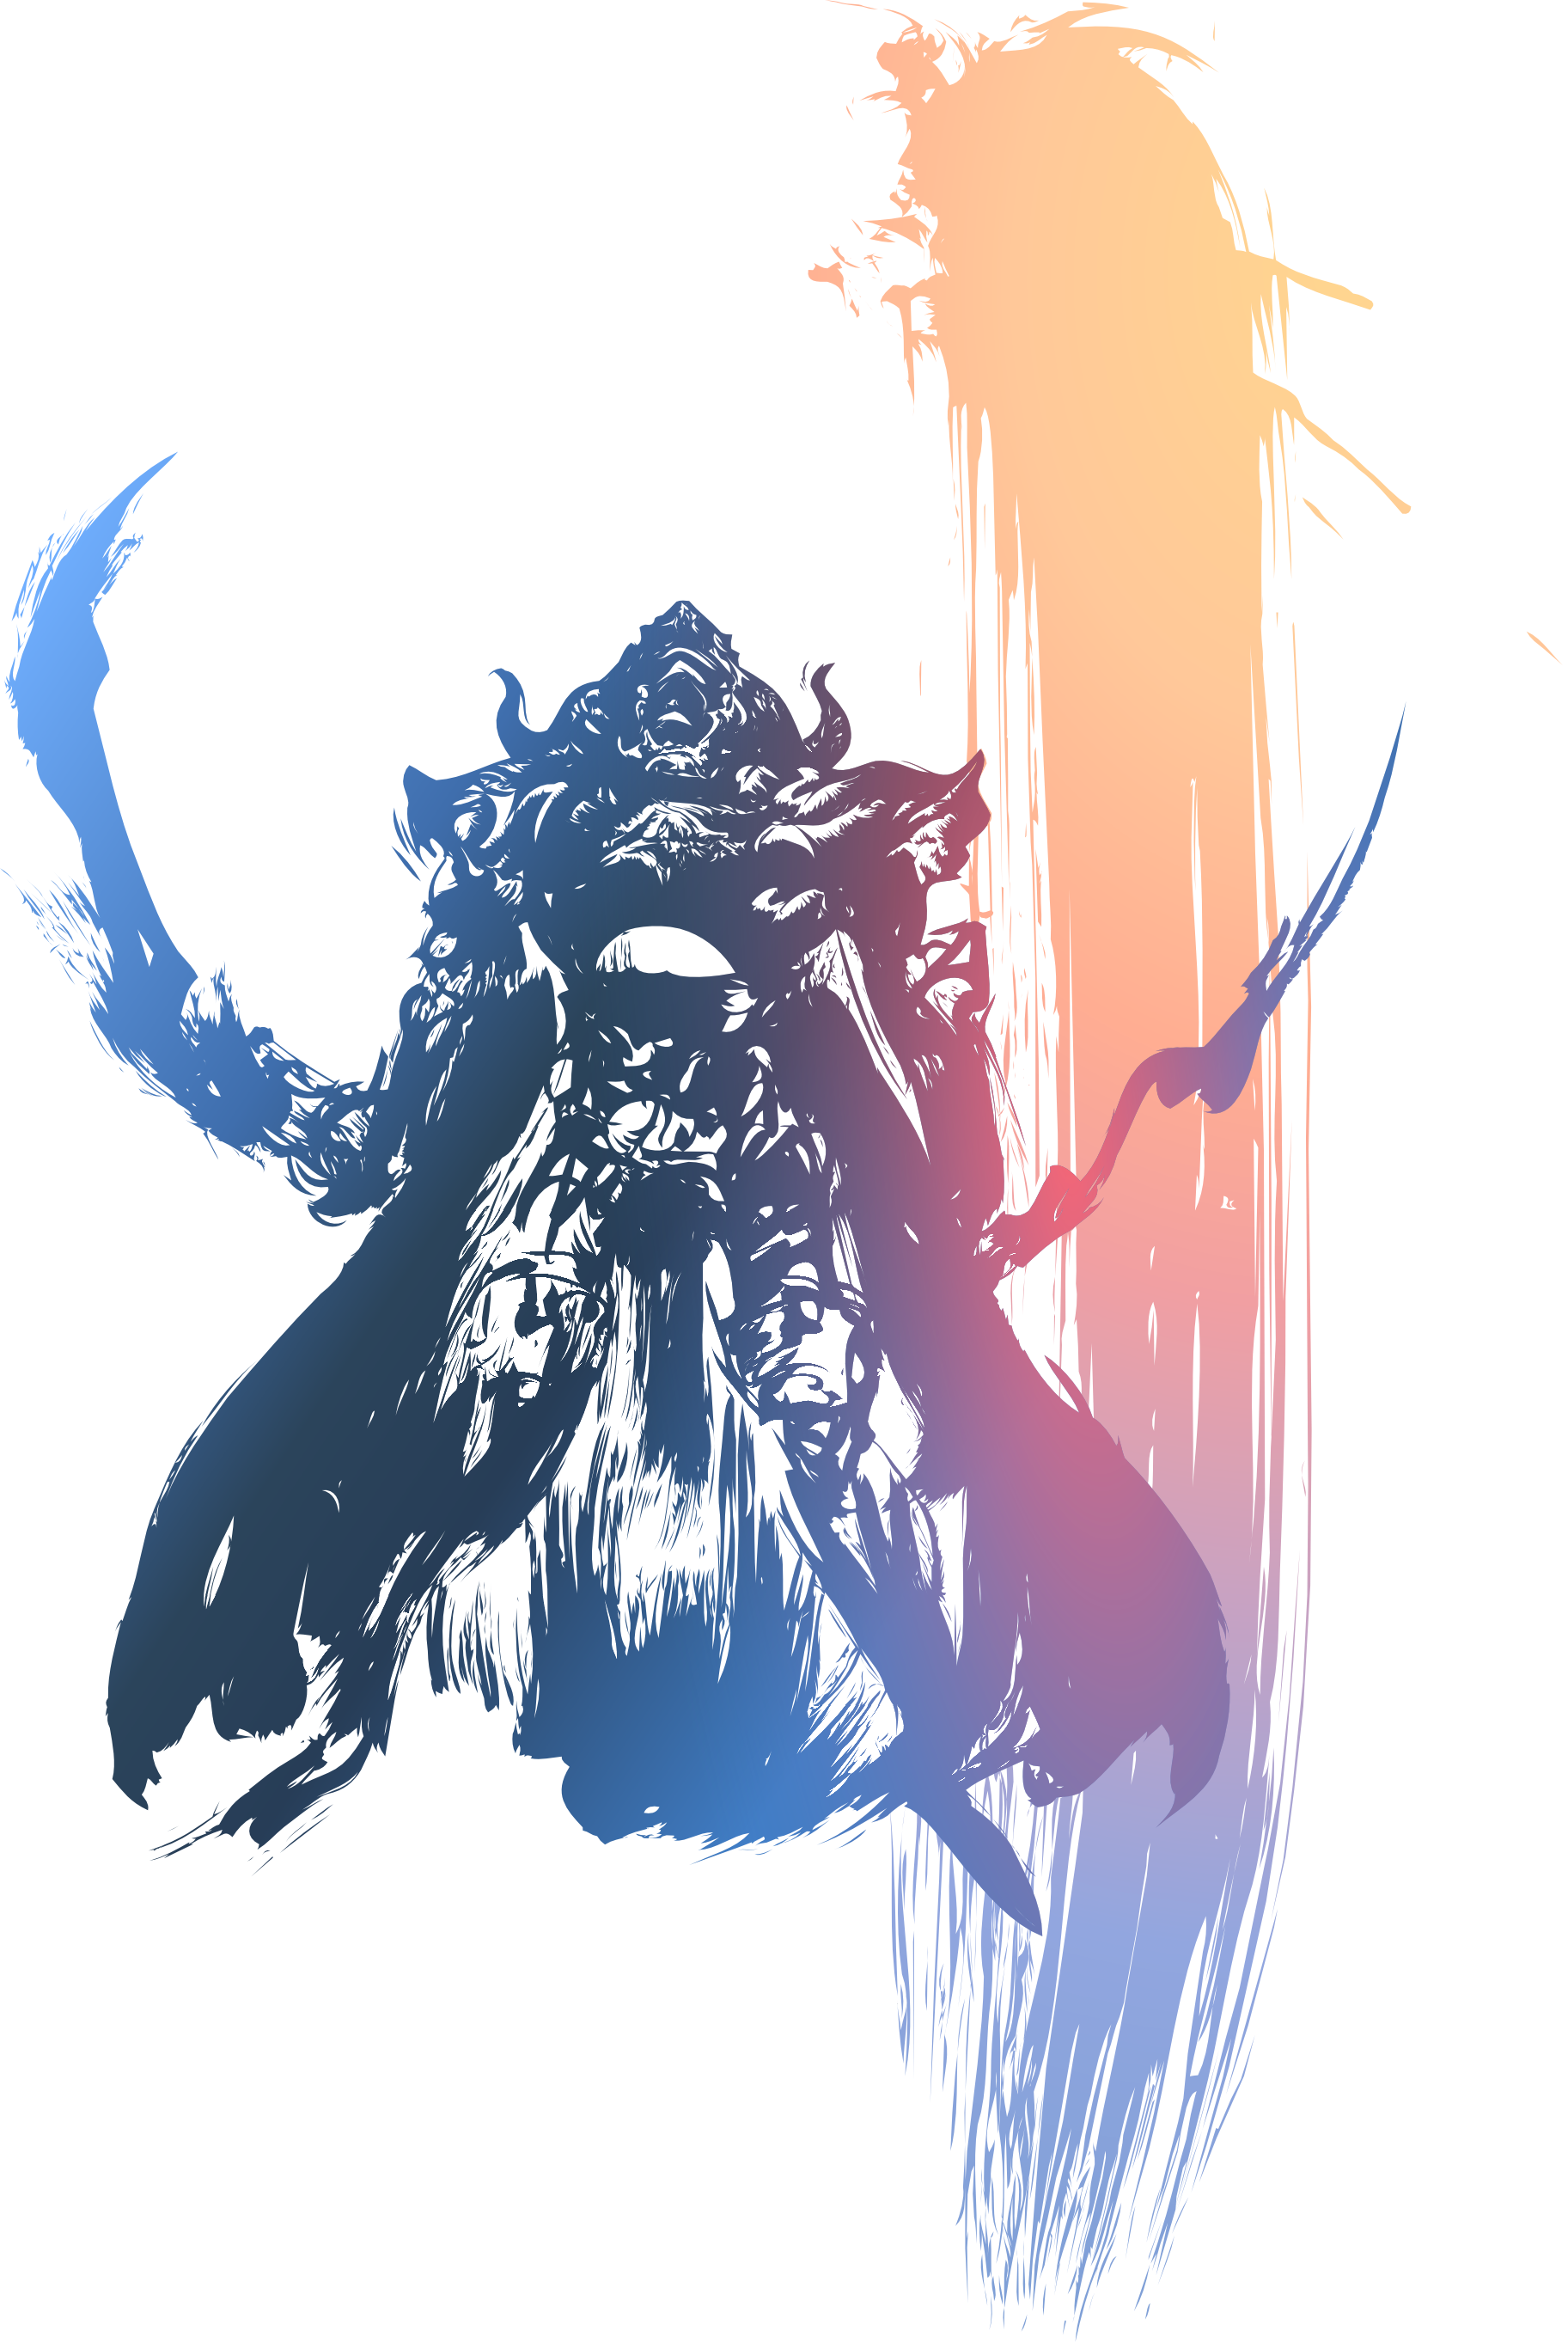
\includegraphics[width=.6\textwidth]{final_fantasy_xii_logo_by_eldi13_d41jlwy}}

\begin{document}
\singlespacing
\maketitle
\tableofcontents
\newpage
\chapter{Introduction}

Welcome to the Final Fantasy X Any\% Speedrun Notes. These notes are the work of a lot of very amazing people who have helped me compile everything here into one document.

Some beginning information about the run:

\begin{itemize}
\item You should be able to complete the first run that you do, as long as you follow the notes exactly. Misreading them can lead to runs that cannot complete. Don't try to do something else because you think it will also work, unless you've tried it before. Examples of this include using Marbles instead of Gems on Biran and Yenke - even though Marbles will still kill, you won't get the overkill which gives us required drops. Information about WHY we do these things are not present in these notes, as they are outside the scope of this document, but if you ask someone will definitely be able to tell you.
\item Common mistakes usually end up being gridding mistakes - some of these are unrecoverable. It sucks, it happens, just realize for next time and double check your grids before doing anything.
\item The run is very long. Make sure you have all the supplies you need.
\item Blitzball sucks. If you lose, it's awful, but the run is still very completable, only loses about 1-2 minutes. Don't worry about it too much.
\item Have fun!
\end{itemize}

Some information about how these notes are laid out:

\begin{itemize}
\item There are a few acronyms used throughout the run.
\begin{itemize}
	\item \sd: \textbf{Skip Dialogue}. During some cutscenes, some of the dialogue is skippable. As soon as the text finishes appearing on the screen, you can hit \textbf{Confirm} to cause it to disappear. This will stop the Voice Over lines from completing, causing the cutscene to progress faster. As a result, you can mash during this to progress faster.
	\item \cs: \textbf{Cutscene}. In game rendered cutscene. Can't do anything about it, just take a break. Usually they will have the approximate time that the cutscenes take, so you can plan your breaks better. These are timed for PS2.
	\item \fmv: \text{Full Motion Video}. Pre-rendered cutscene. Can't do anything about it (usually), just take a break. Usually they will have the approximate time that the cutscenes take, so you can plan your breaks better. These are timed for PS2.
	\item \skippablefmv: \textbf{Skippable Full Motion Video}. Pre-rendered cutscene, but you can skip these if you are on PC. They still have times, because these are not skippable on PS2.
	\item \save: Touching Save Spheres will full heal you. Touch the save sphere, and then cancel out.
\end{itemize}
\item Read each page as such: Left column, then right column, then the next page. There are some instances Read the columns left column first, then right column, then next page. There are some instances where there will be an instruction box that takes up both columns - in this case, do whatever is above the instruction box first (left column, then right column), then do whatever is below the instruction box the same way (left column, then right column)
\item Each bullet point is their own item. Do what it says there before going to the next one.
\item There are instances where you have to get an item, or overdrive, etc before progressing. If the notes say to do so... \textbf{Do So}. These notes don't contain many backup strats.
\end{itemize}

Some information about Spheres:

\begin{itemize}
\item The sphere grid route requires 47 Power Spheres. There are 37 Power Spheres that are guaranteed drops during the course of the run, so you need 10 ``bonus'' spheres in order to be able to complete the run. It will be stated which ones are guaranteed and which values are bonuses. Keep track of the bonuses in order to determine at the stated points if you're low and to do the backup strats then. The guaranteed Power Spheres are:
\begin{itemize}
\item Tros - 2
\item Besaid Dingos - 2
\item Besaid Garuda - 1
\item Geneaux - 2
\item Sahagins - 17
\item Vouivre + Garuda - 2
\item Raldo - 1
\item Bunyip (Mix) - 2
\item Wendigo - 2
\item Bombs - 6
\end{itemize}
\item The sphere grid route requires 17 Speed Spheres. For the most part it doesn't matter when you get them, but keep track of all the ones that you get dropped. There are points to get backup speed spheres that are stated throughout the run.
\ifthenelse{%
		\equal{\blitzresult}{win}
	}{%
		\item These are the \blitzwin\ version of the notes. These notes have the strategies assuming that you have Won Blitzball. If you end up losing Blitzball, then you should switch to the \blitzloss\ set of notes.
	}{%
		\ifthenelse{%
			\equal{\blitzresult}{loss}
		}{%
			\item These are the \blitzloss\ version of the notes. These notes have the strategies assuming that you have Lost Blitzball. If you end up Winning Blitzball, then you should switch to the \blitzwin\ set of notes.
		}{%
			\ifthenelse{%
				\equal{\blitzresult}{both}
			}{
				\item These set of notes contain both the \blitzwin\ and \blitzloss\ strategies. At various points, the strategies that you have to do are different depending on whether or not you won or lost blitzball.
			}{}
		}
	}
\end{itemize}

\newpage
\newpage
\chapter{Prologue}
\begin{enumerate}
	\item Press R3 three times when you have control of the camera.
	\item Talk to Basch, the guard, then open the gate.
	\item When you have control, open the menu
\end{enumerate}
\begin{menu}
	\begin{enumerate}
		\item Battle Mode: Active
		\item Battle Speed: 6
		\item Cursor Positon: Last Selection
	\end{enumerate}
\end{menu}
\begin{battle}{Air Cutter Remora}
	\begin{enumerate}
		\item Thunder x3 while runing in circles
		\item Alternate Attack-Thunder until out of MP
		\item Attack
	\end{enumerate}
\end{battle}
\begin{enumerate}
	\item Proceed up stairs, towards group, up stairs, up stairs.
\end{enumerate}
\begin{battle}{Imperial Guards}
	\begin{enumerate}
		\item Attack each guard twice
		\item Move towards exit while ATB is charging, then back to guards when full for Attack
	\end{enumerate}
\end{battle}
\chapter{Rogue Tomato}
\begin{enumerate}
\item Head \south\ to the shop, \cs. Head \north\ to the bar, go inside.
\item \cs, Select the second option.
\end{enumerate}
\begin{liscense}
\begin{enumerate}
\item Mash
\upl{Accessory 1}
\item \squarec\ Mash
\end{enumerate}
\end{liscense}
\begin{enumerate}
\item Go \south, take the exit opposite the shop.
\item \pickup{small package}{in front of you in the \textbf{Southern Plaza}, by talking to the \textbf{Merchant}}
\item Head to the \textbf{Eastgate} by going \east, \cs
\item Go to the Estersand, \cs
\item Head to the small cliff, fight the \textbf{Rogue Tomato}
\end{enumerate}
\begin{battle}{Rogue Tomato}
\begin{enumerate}
\item Attack
\item Run down the Cliff
\item Attack
\end{enumerate}
\end{battle}
\chapter{Firemane}
\begin{enumerate}
	\item Go back to the \textbf{Eastgate}, talk to \textbf{Kytes}, \cs, \cs, \cs
	\item Head straight \east\ to \lowtown
	\item Go \south\ to the \textbf{South Sprawl}
	\item Go \south\ to \textbf{Old Dalan's Place} on the right, near the next exit, \cs
	\item Exit \south\ to the \textbf{Southgate}, then \south\ to \textbf{Giza}. Pickup \textbf{Potion} from the first chest you see.
	\item \cs, go straight south to the Nomad Villiage.
	\item Talk to the Nomad on the right, near the chest. \cs. Exit through the \south\west.
	\item Head \south\ to the next zone, then \east\ to speak to \textbf{Nomad Youth}
	\item Run around collecting sunstone energy
	\item Go \north\ back to \rabanastre
\end{enumerate}

\begin{equip}
	\begin{itemize}
		\vaanf Remove Armor
		\penelof Remove Everything
	\end{itemize}
\end{equip}
\begin{enumerate}
	\item Go to \lowtown, then go to \textbf{Old Dalan's Place}, \cs. Talk to \textbf{Old Dalan}, \cs, leave, \cs
	\item Head \north\ to the \textbf{North Sprawl}, then take the first exit to the \north-\east\ to the \textbf{Streets of Rabanastre}
	\item Go \south\ to \textbf{Migelo's Sundries}
\end{enumerate}
\begin{shop}{1\,250}
	\sell[exception]{1 Armor, 1 Potion, 1 Teleport Stone, All Phoenix Downs}
	\buy{Phoenix Downs up to 8}
\end{shop}
\begin{enumerate}
	\item Go to the \textbf{Southern Plaza} straight in front of you, then go straight \west\ to the \textbf{Westgate}. Go to the \westersand, \cs
	\item Go to the first \north\east\ exit, then hit yourself down to below 10\% HP. Flee when ATB is at 2/3.
\end{enumerate}

\begin{center}
	\begin{tabular}{|c|c|c|} \hline
	Min HP & Max HP & Action \\ \hline
	      19	& 25&	Punch+Armor\\ \hline
	      26	&26	&Wolf/YOLO Punch+No Armor\\ \hline
	      27	&33	&Punch+No Armor\\ \hline
	      34	&38	&Sword+Armor\\ \hline
	      39	&40	&Punch+Armor x2\\ \hline
	      41	&46	&Punch+Armor, Decide\\ \hline
	      47	&51	&Sword+No Armor\\ \hline
	      52	&56&	Punch+No Armor x2\\ \hline
	\end{tabular}
\end{center}
\begin{enumerate}
	\item Set Battle Speed to Slow
\end{enumerate}
\begin{equip}
	\begin{itemize}
		\vaanf Optimize
	\end{itemize}
\end{equip}
\begin{battle}{Dustia}
	\begin{itemize}
		\item Run over the load line
		\item Run back a bit, positioning yourself near the load line.
		\item \textbf{Dustia} spawns
		\item When the HP bar appears, throw a Phoenix Down on Dustia
		\item Try to pick up whatever drops there are, cross the load line before the EXP from Dustia appears on screen.
		\item Do this 8 times total.
	\end{itemize}
\end{battle}
\begin{enumerate}
	\item Run straight \north, then \north\west to the \textbf{East End}, then take the \lowtown\ entrance \north
	\item Head \north\east\ to the Sewer Entrance, near the brats on the crates
	\item Go into the \waterway, \cs. \save
	\item Follow the path, \flee-ing all the while, until you go up the stairs to the palace. \cs, \cs Can get the chest in the first waterway because it can have remedy/ether
	\item Check for the treasure chests, first the two in the \south\east, then one to the \west, then the \north\east, then the \north\west
	\item Try to get past the guard, then talk to the \textbf{Palace Servant}. Run around the guard, go up the stairs through the door.
	\item Describe shouting stuff to lure guards? \south\west, shout. Back to the entrance, call, then loop around tio the lion - go a bit further, call the guards, then show the sigil to the wall.
	\item In the \textbf{Secret Pasageway}, go straight forward, activate the switch, then go through the suspicious wall.
	\item \cs, mash, \cs.
\end{enumerate}
\begin{liscense}
	\begin{itemize}
		\vaanf
		\begin{itemize}
			\upl{Accessories 2}
			\leftl{Black Magic 1}
		\end{itemize}
	\end{itemize}
\end{liscense}
\begin{gambit}
	\begin{itemize}
		\charactergambit[Off]{\vaan}{\gambitline[enemy]{(Foe: Nearest Visible)}{(Phoenix Down)}}{\gambitdelete}
		\charactergambit{\balthier}{\gambitdelete}{\gambitline[enemy]{Foe: Party Leader's Target}{(Steal)}}
		\charactergambit[Off]{\fran}{\gambitdelete}{\gambitline[enemy]{Foe: Party Leader's Target}{(Fire)}}
	\end{itemize}
\end{gambit}
\begin{enumerate}
	\item \leader{\fran}, \save. Make sure that you fight 2 Ggiantoads.
\end{enumerate}
\begin{battle}{Gigantoad}
\begin{itemize}
\vaanf Fire
\franf Fire
\end{itemize}
\end{battle}
\begin{enumerate}
	\item Go down stairs, \cs
\end{enumerate}
\begin{battle}{Guard Fight}
	\begin{itemize}
		\item \leader{\vaan}
		\franf Fire a guard that isn't the default, targeting whoever is futhest from \ashe
		\vaanf Same as \fran
		\item Make sure that Amalia doesn't get any kills
	\end{itemize}
\end{battle}
\begin{enumerate}
	\item \cs
	\item Use \balthier\ first aid to keep him in place, and \fran\ potion \vaan. Use \vaan\ to \pickup{Leather Shield}{around the corner}. \leader{\fran} to trigger the Flan Fight.
\end{enumerate}
\begin{battle}{Flan}
	\begin{itemize}
		\franf Fire a Flan that isn't the default, by targeting the Flans that are close to Amalia but that she isn't targeting.
		\vaanf Same as \fran
	\end{itemize}
\end{battle}
\begin{enumerate}
	\item \cs. \pickup{Phoenix Down/Red Fang}{next screen}
	\item If Amalia stole a kill, then kill 2 Gigantoads. Otherwise, steal from them with \balthier\ if money is bad, have \fran\ keep on running
\end{enumerate}
\begin{gambit}
	\begin{itemize}
		\vaanf \textbf{OFF}
		\franf \textbf{ON}
		\balthierf \textbf{OFF}
	\end{itemize}
\end{gambit}
\begin{battle}{Firemane}
	\begin{itemize}
		\vaanf Attack
		\balthierf Attack
		\item When Firemane uses bushfire, use a potion to stall. He takes 20\% more damage in the water, but he will teleport to use Bushfire, so you can try to lure him away.
		\item Try to lure and keep Firemane in the water. Can steal with \balthier\ if you need money.
		\item Queue up Fire, by putting the cursor on Black Magic, before the next fight
	\end{itemize}
\end{battle}

\chapter{Mimic Queen}


\begin{battle}{Arena}
\begin{itemize}
\vaanf Mash Fire
\balthierf Attack Daguza
\vaanf Fire another character
\end{itemize}
\end{battle}
\begin{enumerate}
\item If you didn't get the elixer chest, there will be an extra.
\item Do another first aid warp in the clcok tower, after the two chests. Leave \balthier\ at the switch, run down and go to the shop, then touch the switch.
\end{enumerate}
\begin{shop}{400}
\buy{Light Woven Shirt, Blizzard}
\end{shop}
\begin{enumerate}
\item First mimic in first room, first mimic in second room, then steal from the ones you run past.
\end{enumerate}
\begin{battle}{Mimic}
\begin{itemize}
\franf Attack, then Blizzard
\vaanf Attack, then Blizzard
\franf Start running away, let everyone else kill.
\end{itemize}
\end{battle}
\begin{battle}{Flans}
\begin{itemize}
\franf Fire
\vaanf Fire
\end{itemize}
\end{battle}
\begin{liscense}
\begin{itemize}
\balthierf Accessories 1, Black Magic 1
\end{itemize}
\end{liscense}
\begin{enumerate}
\item Tell \balthier\ to cure \vaan\ after killing the Flan to freeze him in place. Use \vaan\ to flick the switch, then \leader{\balthier} to exit the room. \leader{\fran}, keep running.
\item \pickup{Leatherhelm Chest}{right}. Kill 3 mimics, can use \balthier\ Blizzard. Can \pickup{hi-potion}{before the load zone}. \save
\end{enumerate}
\begin{battle}{Mimic Queen}
\begin{itemize}
\item Turn the camera, run backwards to the gate. Blizzard the Mimic Queen with everyone.
\item At the last round: Teleport stone out afterwards.
\begin{equip}
\begin{itemize}
\item Everyone: Remove All
\end{itemize}
\end{equip}
\end{itemize}
\end{battle}
\chapter{Judges}

\begin{shop}{9750}
\begin{itemize}
\item Sell: Everything but Leather Cap, Leather Armor, Lightwove Shirt, 1 Teleport Stone
\item Buy: 39 Phoenix Downs
\end{itemize}
\end{shop}
\begin{enumerate}
\item Blizzard, Fire \vaan\ before Dustia. Optimize All.
\item 	No Armor		Armor	
Punch	49	57	31	38
Blizzard	132	149	110	128
Fire	158	179	133	153
\item Dustia, Gambits, keep on repeating. Do this 39 times, until you get to Level 20.
\item If Dustia heals you, then go back into the Dustia zone, Attack self, then start Fleeing when the ATB is at the first ``T'' in Attack.
\item Potion and run up. If it's sunny you can kill a wolf with Fire, if you need some extra LP. Turn off \vaan\ gambit after Dustia
\item Lots of movement here. (Don't talk to Tomaj - he has 300 gil, 2 potions, 1 teleport stone). Need about 14k gil overall - 14k for things, 5k for Flame Staves if you don't have them dropped. That tells you how much you have extra.
\end{enumerate}
\begin{shop}{800}
\begin{itemize}
\item Sell: All Books of Origins and all Flame Staves except 2
\item Buy: Phoenix Downs until you're comfortable (4 ish)
\end{itemize}
\end{shop}
\begin{enumerate}
\item Killer Bow Chest, in the mines. 15\% chance to get it, worth 1k gil
\item Guaranteed Elixer Chest, 777 Gil
\item Try to get the max number of people per testify - can tell by who turned. Book guy and girl, in the shop get all 4 on the carpet.
\item Party - \vaan, \balthier, \basch
\end{enumerate}
\begin{liscense}
\begin{itemize}
\vaanf Green Magic 1, Time 1, Green 2, Arcane 1
\balthierf Daggers 1, Guns 2, Rods 1, Staves 2, Poles 1
\baschf Poles 1
\end{itemize}
\end{liscense}
\begin{equip}
\begin{itemize}
\item Optimize \basch, \vaan
\end{itemize}
\end{equip}
\begin{enumerate}
\item Fire, Fire, Attack in the first room, then Fire Attack Vossler to put him into Critical.
\end{enumerate}
\begin{battle}{Judges}
\begin{itemize}
\item Flee into the corner to bunch everyone up
\vaanf Attack Judge A
\baschf Attack Judge B
\balthierf If Vossler is below 100 HP, Potion
\item Phoenix Down anyone baut \balthier
\end{itemize}
\end{battle}
\begin{shop}
Buy: Cherry Staff, Dark, Protect, Reflect, Immobilize, Topaki Hat, Killimweave Shirt
\end{shop}
\begin{enumerate}
\item Heal if Vaan is below 400 HP, Balthier if below 300 HP
\item Pickup chests, \leader{\vaan}, Party \vaan, \penelo, \ashe
\end{enumerate}
\begin{liscense}
Check the spreadsheet

Basch	Ashe	Penelo
R1	SmSw1, Stv1	L1
	R1	Stv1
		LA2, MA1, MA2
		Gm15
		PL1 - SplBrkr
		BM1, BM2
		TM1, TM2
		AM1
	WM3-ML25	L1
	Spellbreaker	
	Acc4	
\end{liscense}
\begin{battle}{Judges}
\begin{itemize}
\vaanf Reflect \ashe
\ashef Heal \vaan
\penelof Reflect \penelo
\vaanf Reflect \vaan
\item Battle:
\vaanf Dark Guard B
\penelof Dark Guard B
\ashef Attack \penelo to Red HP
\vaanf Dark \penelo
\penelof Dark \penelo
\end{itemize}
\end{battle}
\chapter{Vossler}

\begin{enumerate}
\item Gambit\ashe\ On. Can use it to heal if anyone is below 70\% and there aren't enemies nearby by stopping to \flee
\item On top of the tower, \vaan\ Reflect \vaan. Reflect on the Bridge before the next fight, \leader{\penelo}. Before the zone line, Reflect Vossler, prepare Dark. Take the Forced Save.
\end{enumerate}
\begin{battle}{Garuda}
\begin{itemize}
\item Reflect \penelo, \ashe
\penelof Dark \ashe
\ashef Attack \penelo
\item Group everyone up before Dark Hits
\end{itemize}
\end{battle}
\begin{shop}{123}
Buy: Cherry Staff (equip on \penelo), 2 Cyrpus Poles, Sleep, Oil, Berserk, Aero
Use Potion on Vaan to freeze him, them remove \ashe, \penelo\ to warp
\end{shop}
\begin{liscense}
\ashe\ BM2
\end{liscense}
\begin{gambit}
\begin{itemize}
\penelof Self-Reflect, Self-Aero
\ashef Self-Aero
\vaanf 1->Steal
\end{itemize}
\end{gambit}
\begin{battle}{Demon Wall}
\begin{itemize}
\item Bring in \ashe, \penelo
\vaanf Run back out of range
\vaanf Protect, Reflect \vaan
\item Once Vossler's reflect wears off, have \vaan Reflect Vossler, turn on \ashe, \penelo\ Gambit, run up
\end{itemize}
\end{battle}
\begin{enumerate}
\item Heal Vossler if near critical. \pickup{elixer}{area}. Make sure \penelo\ has 48 mp
\end{enumerate}
\begin{battle}{Belias}
\begin{itemize}
\vaanf Reflect Vossler, then pick up chest
\vaanf Reflect \vaan
\item 2 rounds, ATB Refresh at the end of the second round
\item Remove All \vaan, \penelo, \ashe, \basch
\item Optimize \basch, \balthier, \vaan, \ashe, \penelo
\end{itemize}
\end{battle}
\begin{enumerate}
\item Setup cursor to Reflect, \penelo\ Gambit On
\end{enumerate}
\begin{battle}{Vossler}
\begin{itemize}
\ashef Aero Guard
\vaanf Reflect \vaan
\penelof Reflect Ashe
\ashef Gambit On
\end{itemize}
\end{battle}
\chapter{Tiamat}

\begin{enumerate}
\item Go to the clan hall, talk to Montblanc to get a lot of items.
\item Buy Traveler
\end{enumerate}
\begin{liscense}
Check Spreadsheet

			R1	Rd1	
				Stv2	
				R1	Rd1
					Stv2
Shld1... HA3					R1
LA5/HA4					
L1					Headsman
R1	Poach				R1
	Traveler				
	GM1				
L1	L1				Bm3
				BM3	L1
			Acc5... Acc8	L1?	
			\end{liscense}

\begin{shop}{Jahara}
\sell{All weapons but Staves, Escutcheon, Bangle, Tourmaline Ring}
\buy{Brigadeen, Red Cap \textit{if you have 23k Gil}}
Can delay this to get the Shielded Armor instead of the Brigadeen next time you're in Jahara.
\end{shop}
\begin{enumerate}
\item Get on Chocobo. When you get off, check for chest, and try to Berserk \basch\ with \penelo\ and then \vaan, then get back on the Chocobo. If you land it, take him out of the part for \balthier.
\item Get on chocobo again, can repeat the berserk before the loading zone.
\vaanf Protect \vaan\ while running, make sure it's up for Tiamate. Larsa has healing gambits, so can stop \flee\ if anyone is below 50\%
\item Cast Traveler, open the Menu to check Step Count. Turn Battle Speed to Min.
\item Battle Speed to Max. Berserk \basch
\end{enumerate}
\begin{battle}{Tiamat}
\begin{itemize}
\item \vaan, \balthier, \basch, Larsa
\vaanf Dark Twice, equip Magicite
\vaanf Phoenix Down x2 Tiamat to draw Tiamat Aggro
\balthierf Check your step counter to make sure that the last 2 digits don't go above whatever you had before, then use Traveler when he flashes Red
\end{itemize}
\end{battle}
\chapter{Mateus}
\begin{menu}
Party: \vaan, \ashe, \penelo
\end{menu}
\begin{equip}
	\begin{itemize}
		\vaanf Remove Mythril Blade, Escutcheon
		\item Optimize \ashe, \penelo
		\baschf Remove All
		\balthierf Remove All
	\end{itemize}
\end{equip}
\begin{shop}{3\,000}
	\sell[everything]{Cherry Staff, Flame Staves, Equipped Armor, Teleport Stones}
	\buy{Fira, Golden Amulet (if can afford), 10-15 Phoenix Down; Max of 1 less than you can afford, Smelling Salts x Max}
\end{shop}
\begin{gambit}
	\begin{itemize}
		      \charactergambit{\vaan}{\gambitline{(Ally: Any)}{(Smelling Salt)}}{\gambitline[enemy]{(Foe: Nearest Visible)}{(Steal)}}
		      \charactergambit{\penelo}{\gambitline{Ally: \penelo}{Reflect (OFF)}}{\gambitline[enemy]{Enemy: Nearest Visible}{(Fira)}}
		      \charactergambit{\ashe}{\gambitline{Ally: \ashe}{(Aero) (OFF)}}{\gambitline[enemy]{Enemy: Nearest Visible}{(Fira)}}
	\end{itemize}
\end{gambit}
\begin{battle}{Jellies}
	\begin{itemize}
		\item 3-4 rooms for Jellies 1, until you have 34 liquids. Reduce this number by 9 per Golden Amulet. To respawn go out of 2 areas. Can toggle \ashe\ gambit on and off to have it target different Jellies. Each room has about 15-20 Jellies. Need 2 Teleport Stones.
		\item If you have Golden Amulet, License and equip on \vaan\ as soon as he has LP for it, usually by the end of the second room.
	\end{itemize}
\end{battle}
\begin{liscense}
	Once 95 LP on Penelo, do the license menu
	\begin{itemize}
		\startLic{penelo}{%
			\rightl {Intercession/Quickening}
			\rightl{Accessories 8}
		}
		\nextLic{ashe}{%
			\item{Accessories 7}
			\upl{Accessories 8}
		}
		\nextLic{vaan}{%
			\item $\downarrow\downarrow$: Accessories 4
			\upl{Accessories 7}
			\upl{Accessories 8}
		}
	\end{itemize}
\end{liscense}
\begin{shop}{123312}
	\sell{Water Magicites, Yellow Liquids}
	\buy{Golden Amulet up to 3; Equip on to \ashe\ + \vaan\ + \penelo, Warp, Confuse, Decoy, Blizzara, 15 Hi-Potions, 10 Phoenix Down}
\end{shop}
\begin{enumerate}
	\item Need 50k Gil after Jellies 2, and 152 LP on \penelo. Can use calculator to determine how many jellies you need, usually about 6~ the second time. Need 5 Teleport Stones afterwards, 1 Float Motes. There are uses for 4 bonus Float Motes.
	\item After jellies, set cursor for \ashe\ to Blizzara, \penelo\ to Immobilize. Turn off \vaan, \ashe, \penelo\ Gambits.
	\item \textit{If you have at least 4 Float Motes:} Float Mote on \vaan\ to go over the traps.
\end{enumerate}
\begin{shop}{7\,500}
	\sell{Water Magicite, Yellow Liquid}
	\buy{Red Cap \textit{if you didn't buy it before}; Equip, 2x Mage's Hat; Equip, Briandine or Shielded Armor; whichever you didn't buy before}
	Should have about 40k Gil remaining
\end{shop}
\begin{menu}
Party: \vaan, \basch
\end{menu}
\begin{liscense}
You need about 160LP on \ashe\ and 190LP on \penelo\ in order to do the full menu.
\begin{itemize}
	\startLic{ashe}{%
		\leftll{Time Magick 2}
		\leftl{Time Magick 3}
		\leftl{Arcane Magick 3, \textit{if you had 160+LP}}
	}
	\nextLic{balthier}{%
		\item $\rightarrow\downarrow\downarrow$: Green Magick 1
		\leftl{Green Magick 2}
		\leftl{Green Magick 3}
	}
	\nextLic{penelo}{%
		\downll{Ether Lore 1}
		\leftl{Magick Lore 40}
		\upl{White Magick 5}
		\item Green Magick 4, \textit{if you had 190+LP}
	}
	\nextLic{vaan}{%
		\item \textit{If you have 190-224 LP:} Libra, Belias
		\item First Aid
		\item $\downarrow\downarrow\leftarrow\leftarrow$: Poach
		\downl{Traveler}
		\leftl{Shield Block}
		\item Remedy Lore 1
		\ifc{As many of these as you can:}{%
			\item Phoenix Lore 1
			\item Potion Lore 2
			\item Spellbound
		}
	}
	\nextLic{ashe}{%
		\item Mystic Armor 2, on bottom left board
		\upl{Mystic Armor 3}
	}
	\nextLic{penelo}{%
		\item Mystic Armor 3
		\rightl{Mystic Armor 5}
	}
	\nextLic{ashe}{%
		\item Mystic Armor 5
	}
\end{itemize}
\end{liscense}
\begin{equip}
\begin{itemize}
\item Optimize \vaan, \penelo, \ashe, \basch
\baschf Dawn Shard
\end{itemize}
\end{equip}
\begin{enumerate}[resume]
	\item Dismount Chocobo before opening door, \leader{\basch}
	\item Turn off \basch\ Gambits
	\item Use Pedestal, with Dawn Shard on your leader
	\vaanf Traver on Guardian. \basch\ \pickup{Megalixir/Elixer}{nearby}. \travelercheck S et Battle Speed to slowest.
	\item In the next room: \vaan\ Potion \vaan, \basch\ Run Away, \vaan\ Potion \basch\ (should never go off). Run a little wide so that \vaan\ stays still, \basch\ touch the Pedestal (With the Dawn Shard equipped). \leader{\vaan}, leave room.
	\item Can heal in the room with the Fake Crystal
	\item In the room after: \basch\ use Phoenix Down x2, Flee once he starts to use the second one. \vaan\ touch the sword, \leader{\basch}
	\item Run past the Bats and the Guardian in the following rooms.
\end{enumerate}
\begin{menu}
\begin{itemize}
\item Party: \vaan, \ashe, \penelo
\battlefast
\end{itemize}
\end{menu}
\begin{gambit}
\begin{itemize}

\vaanf \textbf{OFF}
\ashegambit{Fira}
\penelogambit{Fira}
\item Set all the gambits to OFF %Tyton fix this later
\end{itemize}
\end{gambit}
\begin{enumerate}[resume]
	\ashef Blizzara \penelo
	\penelof Immobilize \ashe
	\item Cursor	Prep Reflect (Vaan)
	\item Can swap leaders to the immobilized characters to despawn enemies.
\end{enumerate}
\begin{battle}{Vinsukur}
	\begin{itemize}
		\vaanf Reflect \ashe, \penelo\ at the stairs.
		\item \GirlsGambitOn
		\vaanf Flee to the corner and stay.
		\item At the end of the fight, \GirlsGambitOff
		\item If Vinuskar pushes the girls, move them away from \vaan.
	\end{itemize}
\end{battle}
\begin{enumerate}[resume]
	\ifc{\ashe\ doesn't have Arcane Magick 3}{%
	 \item Liscense it immediately
	 \penelof Liscense Green Magick 4
	}
	\penelof Action on \vaan (Potion or cure, shouldn't ever go off).
	      \ashef Decoy \vaan
	      \vaanf Touch the statue, then Reflect \vaan
\item \leader{\penelo}, Flee. Once \vaan\ is untargeted:
\end{enumerate}
\begin{menu}
\begin{itemize}
\item Party: \basch, \balthier
\battleslow
\item If \penelo\ doesn't have Green Magick 4, then license it now.
\end{itemize}
\end{menu}
\begin{enumerate}[resume]
	\balthierf Protect \basch
\end{enumerate}
\begin{battle}{Mateus}
	\begin{itemize}
		\item Flee up to Mateus, set the cursor to Green Magic
		\item Party: \vaan, \ashe, \penelo
		\item Equip Dawn Shard onto \vaan
		      \penelof Oil \penelo
		      \item \GirlsGambitOn
		      \vaanf Hi-Potion \vaan, turn on Gambits
		      \item Right before Mateus dies, equip Golden Amulet onto \vaan
		      \item If \ashe\ and \penelo\ have enough MP for another cast, turn off their Gambits
	\end{itemize}
\end{battle}
\chapter{Mandragoras}

\begin{enumerate}
\item \basch, \balthier\ in. Move the armor on \basch.
\item Setup traveler steps before Bergan
\end{enumerate}
\begin{battle}{Bergan}
\begin{itemize}
\vaanf Run up to Bergan
\item Bring in \ashe, \penelo
\begin{liscense}
\begin{itemize}
\item girls: magic 6, magic 6, \vaan\ heavy armor 4-6
\vaanf Traveler
\end{itemize}
\end{liscense}
\end{itemize}
\end{battle}
\begin{shop}{1232}
Buy: 2 Sorc Armor Equip Both, (2 Glacial Staves)
\end{shop}
\begin{enumerate}
\item Remove the Flame Staves from \ashe, \penelo.
\vaanf Traveler the Pumpkin Heads, open the menu to take note of the step count.
\item Use a cure warp with \ashe\ before talking to the Moogle to freeze her by the entrance to the screen.
\ashef Cure herself to make her fall behind
\penelof Blizzara \ashe\, keep running with \vaan\ so that he doesn't get hit, so that they end up in critical. Pull them out of the party. Reflect them when they get to the coast, then put on the Flame Staves.
\end{enumerate}
\begin{shop}{12200}
\begin{itemize}
\item Buy: Mirror Mail, Bio, Dispel
\item 3 Remedies, 10 Hi-Potions
\end{itemize}
\end{shop}
\begin{battle}{Mandragora}
\begin{itemize}
\vaanf Wait for them to gather up, then Traveler them.
\item Use Reflected Firas until they all die.
\end{itemize}
\end{battle}
\chapter{Ahriman}
\begin{menu}
\party{\vaan}
\end{menu}
\begin{enumerate}
	\item Setup Traveler on the first Zombie Knight, making note of your number.
	\item \pickup{Officer's Hat, 12.5\% chance, selling for 3,500}{Somewhere}
	\item Setup a Hi-Potion warp with \basch. Despawn glitch through the area.
\end{enumerate}
\begin{menu}
\party{\vaan, \balthier, \ashe}
\begin{itemize}\item \leader{\balthier}\end{itemize}
\end{menu}
\begin{equip}
\begin{itemize}
\vaanf Remove Mirror Mail
\end{itemize}
\end{equip}
\begin{liscense}
	\begin{itemize}
		\startLic{ashe}{%
			\item Magick Lore 40
			\item Channeling 30
			\item Warmage
			\item Headsman
			\item Swiftness 30
		}
		\nextLic{penelo}{%
			\item CHannelin 30
			\item Warmage
			\item Swiftness 30 \textit{if you got it on \ashe\ as well}
		}
		\nextLic{vaan}{%
			\item Libra
			\item Belias
			\item Poenix Lore 1
			\item Potion Lore 2
			\item Spellbound
			\item Swiftness 30
		}
	\end{itemize}
\end{liscense}
\begin{enumerate}[resume]
	\decoy{\ashe}{\vaan}
	\item \balthier\ can Protect \vaan\ for safety
	\item \vaan\ Hi-Potion
\end{enumerate}
\begin{menu}
\party{\vaan}
\end{menu}
\begin{enumerate}[resume]
\optimize{\vaan}
\item Run past the last group of enemies
\gambiton{\vaan}
\item Enter the fight
\end{enumerate}
\begin{battle}{Ahriman}
\begin{itemize}
\ifc{\enemy{Ahriman} opens with \textbf{Phantasmal Gaze}}
	{
		\item Wait for the animation to start, then continue
	}
\ifc{\vaan\ gets confused}{\item Remove his Weapon}
\begin{menu}
\begin{itemize}
\girlsin
\item \GirlsGambitOn
\end{itemize}
\end{menu}
\vaanf Run behind \enemy{Ahriman} so that \enemy{Ahriman} is facing away from the girls, so that \textbf{Phantasmal Gaze} doesn't hit them.
\item Let exactly 2 \fira s hit \enemy{Ahriman}, 1 per cast off of a single Reflect, not a full round. Letting 3 reset
\atbresetgirls
\battlewait
\gambitoff{\vaan} once he gets a successful scteal.
\item Let a full round of \fira s hit \enemy{Ahriman}, so that a total of 8-9 have hit.
\beliasfreeze\ so that \enemy{Ahriman} doesn't Teleport.
\item Let another full round of \fira s hit, pay attention to who gets off the \fira\ first.
\beliasfreeze{when both caster's ATB reaches the ``F'' in \fira}
\item After the \fira s are done, then:
\begin{itemize}
\item Whoever got the first \fira\ off (usually \penelo): Hi-Potion \enemy{Ahriman}
\item Whoever got the second \fira\ off (usually \ashe): Warp Mote
\vaanf Steal \enemy{Ahriman}
\end{itemize}
\item \enemy{Ahriman} Teleports
\vaanf Run behind \enemy{Ahriman}, paying attention to which way that he's facing.
\begin{menu}
\begin{itemize}
\girlsout
\gambitoff{Turn the Hi-Potion user's}
\end{itemize}
\end{menu}
\item Close the menu and immediately reopen it
\begin{menu}
\begin{itemize}
\girlsin \gambiton{Turn the Hi-Potion user's}
\end{itemize}
\end{menu}
\item Do another round of \fira s
\beliasfreeze{the same way that you did before.}
\item After the damage lands:
\begin{menu}
\begin{itemize}
	\item ATB Reset everyone by removing their Armor and then Optimizing them all
	\item Config: Battle Speed Slowest \textit{if Swiftness is on both girls else} Battle Speed Second Slowest
\end{itemize}
\end{menu}
\item Let the \fira s charge slowly.
\item As soon as \enemy{Ahriman}\ teleports to you briefly:
\begin{itemize}
\beliasfreeze{should be about when the ATB is charged to the ``r'' in \fira}
\end{itemize}
\item Once \enemy{Ahriman} dies, \GirlsGambitOff
\end{itemize}
\end{battle}
\begin{enumerate}[resume]
\item Config: Battle Mode Active
\item \pickup{Elixir (100\%), Gaia Hat/Elixir (50/50)}{in the room}
\end{enumerate}
\chapter{Cid}


\begin{liscense}
BM4, BM4 on the girls

GM1 on another girl

\vaan\ switfness
\end{liscense}
\begin{gambit}
\begin{itemize}
\ashegambit{Bio}
\penelogambit{Bio}
\end{itemize}
\end{gambit}
\begin{shop}{123}
\buy{Aeroga}
\end{shop}
\begin{enumerate}
\item Remove \vaan\ armor, protect him with \penelo
\item Get the girls down to crit with Blizzara. Decoy \vaan\ by removing the armor, then re-equip and take him out of the party.
\item Optimize everyone, turn on gambits
\end{enumerate}
\begin{battle}{Cid}
\begin{itemize}
\item Move everyone up to try and reflect onto a single Rook.
\vaanf Hi-Potion to try at full as much as possible. Can use an Elixir.
\item After you kill the first Rook:
\ashef Target Rook C
\penelof Target Rook C
\vaanf ATB Reset, Traveler on Rook
\item Let the girls kill
\end{itemize}
\end{battle}
\chapter{Rafflesia}

\begin{enumerate}
\item Remove \vaan\ armor, protect him with \penelo
\item Get the girls down to crit with Blizzara. Decoy \vaan\ by removing the armor, then re-equip and take the girls out of the party.
\item Optimize everyone, turn on gambits, switch Bio to Aeroga
\end{enumerate}
\begin{battle}{Rafflesia}
\begin{itemize}
\vaanf Run up
\item Bring the girls in
\item Turn the gambits off when the fight is about to end.
\end{itemize}
\end{battle}
\chapter{Daedalus}

\begin{enumerate}
	\vaanf Remedy \vaan, if he didn't block Nectar Volley
	\penelof Dispell Penelo
	\ashef Hi-Potion \vaan\ if needed
	\item Remove \ashe\ from the Party.
	\item On the next screen, \penelo\ Immobilize \penelo.
	\item On the next two screens, switch party leader to \penelo\ in order to despawn enemies. Look for the illusions in order to find the right path.
	\item At the start of the last screen, have \penelo\ do an action onto \vaan\ to trigger the ``too far away'' trick.
	\item Summon Belias to open the door.
\end{enumerate}
\begin{menu}
	\party{\balthier, \ashe, \penelo}
\end{menu}
\begin{equip}
	\begin{itemize}
		\optimize{\penelo, \ashe}
	\end{itemize}
\end{equip}
\begin{gambit}
	\begin{itemize}
		\ashegambit{Bio}
		\penelogambit{Bio}
	\end{itemize}
\end{gambit}
\begin{battle}{Daedalus}
	\begin{itemize}
		\penelof Dispell \ashe
		\penelof Reflect \penelo
		\ashef Reflect \balthier
		\ashef Reflect \ashe
		\balthierf Spam Confuse on \enemy{Daedalus} and run in circles to regenerate MP
		\item Once close enough, \GirlsGambitOn
		\item At the end of the battle, \GirlsGambitOff
	\end{itemize}
\end{battle}
\chapter{Tyrant}

\begin{liscense}
RL3, Swiftness					
L1					Ch50... Sw50
					ML55
				Ch50...Sw50	L1
				ML55	
AM2				R1	R1

Check the spreadsheet
\end{liscense}
\begin{gambit}
\begin{itemize}
\ashegambit{Blizzara}
\penelogambit{Blizzara}
\end{itemize}
\end{gambit}
\begin{enumerate}
\item Immobilize warp/despawn throughout this area.
\item Reflect \ashe, \penelo\ after the door
\end{enumerate}
\begin{battle}{Tyrant}
\begin{itemize}
\penelof Dispel
\vaanf Once it's charged a bit, start spamming Confuse
\item Try to keep the girls a bit away, and keep him confuse looped.
\end{itemize}
\end{battle}
\chapter{Shemhazai}

\begin{enumerate}
\item Heal \vaan to full
\vaanf Protect \vaan
\penelof Reflect \vaan
\ashef Decoy \vaan
\item Gambits on for the Girls. take the girls out of the party
\end{enumerate}
\begin{battle}{Shemhazai}
\begin{itemize}
\item Bring the girls back in.
\begin{gambit}
\begin{itemize}
\ashegambit{Bio}
\penelogambit{Bio}
\end{itemize}
\end{gambit}
\vaanf Immobilize Shemhazai
\vaanf Belias Freeze whiel the Bios are hitting. Start when they charge, stop when the numbers disappear.
\vaanf Traveler at the very end.
\end{itemize}
\end{battle}
\chapter{Hydro}

\begin{equip}
	\begin{itemize}
		\vaanf Remove Mirror Mail
		\penelof Remove Golden Amulet, Glacial Staff
		\ashef Remove Golden Amulet, Glacial Staff
	\end{itemize}
\end{equip}
\begin{liscense}
	\begin{itemize}
		\startLic{balthier}{\item Nothing}
		      \nextLic{penelo}{\item Black Magick 5 \item Quickening}
		      \nextLic{ashe}{\item Black Magic 5 \item Shemhazai \ifc{If can afford}{\item Headsman \item Swiftness \item Spellbound}}
		      \nextLic{penelo}{\item Channeling 80 \ifc{If you also got them for \ashe}{\item Headsman \item Swiftness \item Spellbound}}
		      \nextLic{vaan}{\item Remedy Lore 3 \item HP+200}
	\end{itemize}
\end{liscense}
\begin{enumerate}
	\item Once you get to Balfonheim
\end{enumerate}
\begin{shop}{123123}
	\begin{itemize}
		\item Magick Shop:
		      \sell[everything]{Armor, Flame Staves, Cherry Staves}
		      \buy{Firaga}
		\item Item Shop:
		      \buy{X-Potions, Phoenix Downs}
		\item Spend all of your money, and get as mnay healing items as you can. Having at least 10 of each X-Potions and Phoenix Downs is recommended. You can also buy some extra Remedies and Gold Needles if you have extra money; Gold Needles you're usually fine without one, but having an extra Remedy can be useful.
	\end{itemize}
\end{shop}
\begin{enumerate}
	\item Once you get to Ridorana:
	\item Run past enemies on the next two screens.
	      \ashef Reflect Reddas
	\item Once \ashe\ catches up:
	      \begin{itemize}
		      \penelof \fira \ashe
		      \ashef Reflect \ashe
	      \end{itemize}
	\item Continue onto the next screen.
	      \penelof Reflect \penelo
	      \decoy{\ashe}{\vaan}
	\item \castprotect{\vaan}{\vaan}
	\item Set your Cursor onto Green Magic, Oil
\end{enumerate}
\begin{menu}
	\party{\vaan, Reddas}
\end{menu}
\begin{equip}
	\begin{itemize}
		\optimize{\vaan, \penelo, \ashe}
	\end{itemize}
\end{equip}
\begin{battle}{Hydro}
	\begin{itemize}
		\vaanf Run Close, then once \vaan gets targeted:
		\girlsin

		\begin{gambit}
			\begin{itemize}
				\ashegambit{Firaga}
				\penelogambit{Firaga}
			\end{itemize}
		\end{gambit}
		\penelof Oil the party
		\item Wait until \enemy{Hydro} doesn't use Countdown, Bile, Fireball, or Darkra.
		      \vaanf Once he aggros onto \vaan, he will start walking towards \vaan. Run around in a circle while keeping the camera focused to run loop de loops, keeping \ashe, \penelo\ between \vaan\ and \enemy{Hydro} and let them kill.
		\item After the last round of Firagas go off, then \GirlsGambitOff Flee.
	\end{itemize}
\end{battle}
\chapter{Pandemonium}

\begin{battle}{Pandemonium}
\begin{itemize}
\item Bring the girls in
\begin{gambit}
\begin{itemize}
\charactergambit[Off]{\ashe}{\gambitline{Ally: \ \ashe\ \ }{Reflect}}{\gambitline{Ally: \ \ashe\ \ }{(Aerora)}}
\end{itemize}
\end{gambit}
\penelof Immobilize Reddas
\ashef Gambit On at the end after Immobilization.
\vaanf Confuse lock Pandemonium
\penelof Aero, then Aerora
\end{itemize}
\end{battle}
\chapter{Slyt}

\begin{enumerate}
	\item Take the girls out of the party.
\end{enumerate}
\begin{liscense}
	\ashe Channeling, Dispel
\end{liscense}
\begin{battle}{Brainpans}
	Roosta TODO
\end{battle}
\begin{enumerate}
	\item Reflect the girls
	\item Gambits to Firaga
\end{enumerate}
\begin{battle}{Slyt}
	\begin{itemize}
		\item Let the girls kill. Dispel the girls after the fight.
	\end{itemize}
\end{battle}
\chapter{Fenrir}

\begin{enumerate}
	\item Reflect both girls by toggling gambits, then take them out of the party.
	\item Battle speed up, bring in \balthier, \ashe, \penelo
\end{enumerate}

\begin{gambit}
	\begin{itemize}
		\ashegambit{Bio}
		\penelogambit{Bio}
	\end{itemize}
\end{gambit}
\begin{enumerate}
	\item \leader{\balthier}
	\item Immobilize on Reddas, Reflect on the Girls. \ashe\ Decoy \balthier, gambits on
	\item Put the cursor on sleep
\end{enumerate}
\begin{battle}{Fenrir}
	\begin{itemize}
		\balthierf Run backwards diagonal, spam Sleep
		\item Keep him away from Reddas
		      \balthierf Traveller
		      \balthierf Attack \balthier\ until he's below 120 HP
	\end{itemize}
\end{battle}
\chapter{Hashmal}

\begin{liscense}
Magic, Lore, Channeling on the girls
\vaan HP+500, Battle Lore
\end{liscense}
\begin{enumerate}
\item Take off the mirror mail, have one of the girls use a float mote. Protect \vaan, battle sleep to minimum.
\item Reflect Reddas, Bring the girls back in, Aerogas Gambits on the Girls
\end{enumerate}
\begin{battle}{Hashmal}
Belias Freeze, ATB Reset.
\end{battle}
\chapter{The Undying}
\begin{enumerate}
	\item Decoy Vaan, Reflect Girls. Make sure that Reddas is in Crit, Berserk him.
\end{enumerate}
\begin{gambit}
	\begin{itemize}
		\ashegambit{Firaga}
		\penelogambit{Firaga}
	\end{itemize}
\end{gambit}
\begin{battle}{Cid}
	\begin{itemize}
		\item ROOSTA TODO
	\end{itemize}
\end{battle}
\begin{battle}{Undying}

\end{battle}
\end{document}